\section{LSM-деревья}

Подход LSM-деревьев был предложен в статье~\cite{LSM}. Основная идея лежащая в
основе LSM-деревьев заключается в том, что изменения индексной структуры
накапливаются в памяти, после чего большими порциями выписываются на диск в
отсортированном порядке и по возможности последовательно. Дополнительно к
основному алгоритму в~\cite{BLSM} описываются несколько оптимизаций и
модификаций, которые позволяют сделать LSM-деревья более дружелюбными по
отношению к запросам на чтение. Далее в этом разделе описывается вариация
LSM-деревьев использованная в данный момент в реализации myfs.


\subsection{Структура LSM-деревьев}

LSM-дерево состоит из нескольких уровней, который далее будут обозначаться как
$C_i$, где $i$ - это целое неотрицательное число, которое обозначает номер
уровня. Уровни $C_0$ и $C_1$ - это уровни которые хранятся в памяти. Все
остальные уровни ($C_i$, где $i > 1$) хранятся на диске. Количество уровней
фиксировано и никогда не изменяется\footnote{Побочный эффект такого ограничения
это логарифмическая сложность поиска, однако основной причиной этого ограничения
является не алгоритмическая сложность, а простота реализации.}. Каждый уровень
представляет из себя упорядоченный словарь.


\subsubsection{Операции над LSM-деревом}

Все операции обновления индекса (вставка и удаление ключей) всегда выполняются
над уровнем $C_0$. Если операция вставки не вызывает вопросов, то операция
удаления ключа требует пояснений так как LSM-дерево состоит из нескольких
словарей. Операция удаления ключа заключается в добавлении этого ключа со
специальным маркером, который будет обозначать, что этот ключ удален. В
последствии ключи с таким маркером будут удалены из дерева.

По мере работы над LSM-деревом ключи будут переходить от уровней с меньшими
номерами в уровни с большими номерами посредством выполнения операции слияния.
Таким образом для поиска ключа в LSM-дереве необходимо выполнить поиск
последовательно на каждом уровне начиная с 0 до тех пор пока ключ не будет
найден. Если при этом у ключа присутствует маркер-признак того, что ключ был
удален, то значит в LSM-дереве искомый ключ отсутствует. При выполнении запросов
возвращающих ключи в некотором диапазоне придется просмотреть все уровни и
объединить результаты из каждого из этих уровней.


\subsubsection{Перенос данных из памяти на диск}

По мере выполнения операций вставки и удаления словарь $c_0$ в памяти может
стать очень большим, и в какой момент может потребоваться сохранить данные из
памяти на диск. Эта операция называется flush и она выполняется в два этапа:
\begin{itemize}
  \item $C_0$ переносится в $C_1$, а словарь $C_0$ инициализируется пустым
        множеством пар;
  \item над словарями $C_1$ и $C_2$ выполняется операция слияния, которая
        создает новый словарь.
\end{itemize}

Перенос из $C_0$ в $C_1$ требуется для того, чтобы не блокировать операции
записи на время сохранения данных на диск. Перенос $C_0$ в $C_1$ фактически
сводится к подмене нескольких указателей в памяти, т. е. выполняется довольно
быстро. После этого можно продолжать выполнение операций вставки/удаления над
новым пусты $C_0$, в то время как $C_1$ остается неизменным во время выполнения
операции слияния.

Кроме того, разделение на два этапа требуется для эффективного создания
контрольной точки файловой системы на диске с минимальными задержками для
пользователей. Подробнее о реализации создании контрольной точки и использовании
flush рассказывается в разделе~\ref{sec:commit}.


\subsection{Слияние деревьев}

Ключевой в работе LSM-деревьев является операция слияния подробнее рассмотренная
ниже. Как уже упоминалось выше слияние выполняется, если $C_0$ в памяти стал
слишком большим. Однако, если поддерживать только 3 уровня $C_0$,
вспомогательный $C_1$ и $C_2$, то по мере роста размера индекса выполнение
операции слияния будет занимать слишком много времени, так как слияние требует
последовательного прохода по обеим сливаемым последовательностям.

Действительно, если $C_2$ будет расти неограниченно, то его размер начнет
доминировать время выполнения слияния. Фактически в этом случае на каждое
слияние $C_1$ и $C_2$ придется вычитывать и перезаписывать большую часть
индекса. Чтобы этого избежать этого в myfs размер $C_2$ ограничивается так,
чтобы слияние можно было выполнять сравнительно быстро.


\subsubsection{Ограничения на размеры уровней}
\label{sec:lsmlev}

В текущей реализации используется ограничение в 2Mb на размер $C_2$. При
превышении ограничения уровень $C_2$ будет слит с уровнем $C_3$. Всего уровней
6: $C_0$ и $C_1$ в памяти, $C_2$ - $C_5$ на диске. Размеры уровней на диске
образуют геометрическую прогрессию с основанием 4. Т. е. размер уровня $C_3$
ограничен 8 Mb, размер уровня $C_4$ 32 Mb, а последний уровень $C_5$ не имеет
ограничения так как его уже нескем сливать.

Количество деревьев было выбрано из следующих соображений. В типичной домашней
файловой системе может содержаться порядка миллиона файлов и каталогов. Простой
скрипт на языке Python:

\begin{lstlisting}[language = Python]
#!/usr/bin/env python

import os

total_len, total_size, nitems, nfiles = 0, 0, 0, 0
for path, dirs, files in os.walk('/'):
    to_remove = []

    for name in dirs:
        fullname = os.path.join(path, name)
        # exclude pseudo filesystems
        if fullname in ('/sys', '/proc', '/media'):
            to_remove.append(name)
            continue
        total_len += len(name)

    for name in to_remove:
        dirs.remove(name)

    for name in files:
        fullname = os.path.join(path, name)
        total_len += len(name)
        if not os.path.islink(fullname) and os.path.isfile(fullname):
            total_size += os.stat(fullname).st_size
            nfiles += 1

    nitems += len(dirs) + len(files)

print 'entries: {}, avg size: {}, avg len {}'.format(nitems,
    total_size / nfiles, total_len / nitems)
\end{lstlisting}
Запущенный на компьютере автора демонстрирует, что суммарное количество записей
во всех каталогах (включая символьные и жесткие ссылки) чуть более полумиллиона,
а средний размер имени всего 15 байт. Служебная информация с учетом имени,
которая хранится для каждой такой записи в файловой системе myfs занимает
порядка 54 байт, таким образом 6-и уровней достаточно чтобы сохранить всю
информацию о структуре каталогов и иметь некоторый запас.


\subsubsection{Операция слияния}

Операция слияния выполняется над двумя последовательными словарями $C_i$ и
$C_{i+1}$ в результате создавая новый словарь $C'_{i+1}$ на диске, содержащий
элементы $C_i$ и $C_{i+1}$. После завершения слияния словари $C_i$ и $C_{i+1}$
больше не требуются, словарь $C_{i+1}$ подменяется новым словарем $С'_{i+1}$,
а словарь $C_i$ подменяется пустым словарем.

Так как все словари поддерживают данные в упорядоченном виде\footnote{Можно
также отсортировать пары ключ/значения из словаря перед слиянием}, то слияние
требует одного прохода по каждому словарю и выполняется за линейное от
количества пар время подобно операции слияния в алгоритме сортировки слиянием.

При слиянии однако требуется специальная обработка одинаковых ключей. Например,
в ситуации, когда $C_i$ и $C_{i+1}$ содержат один и тот же ключ, но ключ из
$C_i$ содержит маркер-признак удаленного ключа, то в результирующий словарь
должен попасть только ключ с этим маркером. Таким образом в случае совпадения
ключей из $C_i$ и $C_{i+1}$ в результирующий словарь $C'_{i+1}$ попадает только
более новый ключ из $C_i$.

Более того, если $C_{i+1}$ является последним используемым уровнем в дереве и
ключ содержит маркер-признак удаленного ключа, то мы можем не добавлять его в
результирующее дерево. Таким образом дойдя до последнего уровня в дереве ключ
с маркером удаляется из LSM-дерева физически.


\subsection{Словарь в памяти}

В качестве словаря в памяти (для уровней $C_0$ и $C_1$) используется lock-free
реализация структуры данных известной как SkipList~\cite{SKIP}.


\subsubsection{Интерфейс словаря в памяти}

Словарь в памяти должен поддерживать интерфейс описываемый структурой
myfs\_mtree из inc/lsm/lsm.h:
\begin{lstlisting}
struct myfs_mtree {
    int (*insert)(struct myfs_mtree *, const struct myfs_key *,
                  const struct myfs_value *);

    int (*lookup)(struct myfs_mtree *, struct myfs_query *);
    int (*range)(struct myfs_mtree *, struct myfs_query *);
    int (*scan)(struct myfs_mtree *, struct myfs_query *);

    size_t (*size)(const struct myfs_mtree *);
};
\end{lstlisting}

В этой структуре есть только одна операция модификации - insert. Благодаря тому,
что данные реально не удаляются, вместо этого вставляются ключи со специальным
маркером не требуется поддерживать специально операцию удаления, что упрощает
также реализацию lock-free алгоритма, так как не требуется заботиться о
безопасном освобождении памяти при удалении ключей\footnote{Все еще нужно уметь
освобождать дерево целиком после того, как его содержимое было сохранено на
диск. О том, как это организовано рассказывается дальше.}.

Далее идут три операции поиска:
\begin{itemize}
    \item lookup - точечный поиск одного значения удовлетовряющего некоторому
          предикату, согласующемуся с порядком хранения элементов в словаре;
    \item range - запрос поиска всех значений входящих в некоторый диапазон
          заданный некоторым предикатом, согласующимся с порядком хранения
          элементов в словаре;
    \item scan - поиск всех элементов, удовлетворяющих некоторому произвольному
          предикату.
\end{itemize}

Во всех случаях предикат задается как в виде структуры myfs\_query определенной
в inc/types.h:
\begin{lstlisting}
struct myfs_query {
    int (*cmp)(struct myfs_query *, const struct myfs_key *);
    int (*emit)(struct myfs_query *, const struct myfs_key *,
                const struct myfs_value *);
};
\end{lstlisting}

В этой структуре поле cmp проверяет удовлетворяет ли значение предикату. Эта
функция должна возвращать 0, если переданный ключ удовлетворяет предикату, -1
если переданный ключ меньше искомого и 1 если больше. Функция emit вызывается
для каждой пары ключ значение, которые удовлетворяют заданному предикату.

Последняя часть интерфейса словаря в памяти - это функция size. Функция должна
возвращать примерное количество записей в словаре. Эта функция используется
чтобы проверить необходимость сохранения словаря на диск.


\subsubsection{Разрешение коллизий в словаре в памяти}

При работе со словарем в памяти один и тот же ключ может быть добавлен несколько
раз. Например, чтобы удалить ключ из LSM-дерева этот ключ добавляется в дерево
со специальным маркером. В такой ситуации, вместо того чтобы изменять элемент
уже хранящийся в SkipList-е в словарь добавляется новый элемент. Изменение уже
хранящегося элемента не желательно так как он может в данный момент
использоваться, например, при конкурентом запросе на поиск. Эту проблему можно
преодолеть используя техники безопасного освобождения памяти, такие как RCU или
Hazrd Pointer, но в целях простоты реализации было решено использовать другой
подход.

Используемый подход заключается в добавлении к элементу уникального
идентификатора. Причем идентификаторы по мере работы с SkipList-ом монотонно
возрастают. Элементы с большим идентификатором, т. е. более новые, считаются
меньше элементов с меньшим идентификатором, если ключи элементов равны. Таким
образом благодаря идентификатору всегда можно понять какой элемент является
последней версией.


\subsection{Словарь на диске}

Словарь на диске создается при выполнении операции слияния. После того как
словарь был создан он никогда не изменяется, но может быть в будущем заменен
новым словарем.

В качестве словаря на диске используется сильноветвистое идеально
сбалансированное дерево поиска подобное B+ дереву. Выбор структуры обусловлен
двумя факторами:
\begin{itemize}
  \item в таком дереве поиска легко искать значения по ключу не читая его в
        память целиком, в отличие, например, от классических SSTable,
        часто используемых при реализации LSM-деревьев;
  \item создавать такое дерево из отсортированного потока элементов не сильно
        сложнее чем SSTable, так как достаточно всего лишь одного прохода по
        отсортированной последовательности элементов.
\end{itemize}


\subsubsection{Интерфейс словаря на диске}

Словарь на диске поддерживает операции похожие на операции словаря в памяти за
исключением операции scan. Кроме того, так как словарь на диске никогда не
изменяется, после того как был создан, то дополнительно реализован интерфейс
итераторов. Изменение интерфейса обусловлено несколькими обстоятельствами:
\begin{itemize}
  \item полный просмотр словаря на диске требуется только при выполнении
        операции слияния и использовать итератор для этого удобнее так как
        необходимо сканировать два словаря одновременно;
  \item при выполнении запросов на диапазоне требуется просмотр каждого словаря
        на диске, используя итераторы легко реализовать запросы на диапазоне без
        загрузки всего диапазона целиком в память;
  \item реализовать scan, если потребуется, легко используя итератор, а вот
        обратное сделать тяжелее, если предполагать, что словарь на диске может
        не поместиться в память.
\end{itemize}

\subsubsection{Структура словаря на диске}

Каждый узел дерева на диске начинается со структуры \_\_myfs\_ctree\_node\_sb
описанной в файле inc/lsm/ctree.h:
\begin{lstlisting}
struct __myfs_ctree_node_sb {
        le32_t items;
        le32_t size;
} __attribute__((packed));
\end{lstlisting}

Структра хранит число элементов и количество байт, которые занимает узел дерева.
Далее следую собственно элементы, хранящиеся в узле дерева, перед каждым
элементом хранится структура \_\_myfs\_ctree\_item:
\begin{lstlisting}
struct __myfs_ctree_item {
        le32_t key_size;
        le32_t value_size;
} __attribute__((packed));
\end{lstlisting}
Каждый элемент состоит из пары ключ и значение, размеры ключа и значения в
байтах и хранятся в этой структуре.

В листьях дерева хранятся ключи и значения добавленные в дерево, во внутренних
узлах хранятся только ключ, а вместо настоящих значений хранятся указатели на
дочерние листы дерева (файл inc/types.h):
\begin{lstlisting}
struct __myfs_ptr {
    le64_t offs;
    le64_t size;
    le64_t csum;
} __attribute__((packed));
\end{lstlisting}

В указателе на каждый узел дерева хранится 64-битная контрольная сумма, чтобы
иметь возможность проверять целостность узла. Указатель на корень дерева, а
также некоторая дополнительная информация сохраняются в структуре
\_\_myfs\_ctree\_sb:
\begin{lstlisting}
struct __myfs_ctree_sb {
    struct __myfs_ptr root;
    le32_t size;
    le32_t hight;
} __attribute__((packed));
\end{lstlisting}


\subsubsection{Построение словаря на диске}

Как отмечалось выше построение словаря на диске может быть выполнено за один
проход по отсортированной последовательности элементов. Во время построения
словаря на диске алгоритм поддерживает данные на нескольких уровнях. Новые
элементы добавляются на 0-ой уровень. Этот уровень соответствует листьям дерева
поиска. Когда нулевой уровень заполняется он выписывается на диск как узел
дерева, при этом на уровень 1 добавляется новый элемент состоящий из наибольшего
ключа выписанного узла дерева и указателя на этот узел (структура
\_\_myfs\_ptr). По мере заполнения уровня 1 данные этого уровня также будут
выписаны на диск в качестве узла дерева и новый элемент будет добавлен на
уровень 2. Этот процесс продолжается пока не будут обработаны все элементы
входной последовательности.

При выписывании дерева контролируется его ветвистость. В текущей реализации
узел выписывается только если количество элементов в нем не менее 16 либо
если больше нет элементов для добавления в дерево. 


\subsection{Выбор ветвистости дерева}

В текущей реализации ветвистость дерева определяется следующим образом:
\begin{itemize}
  \item узел с менее чем 16 ключами выписывается только в том случае, если не
        осталось элементов для добавления в дерево;
  \item если в узле уже есть 16 элемента и размер узла выровненный на ближайшую
        сверху границу страницы позволяет добавлять ключи, то ключи добавляются
        в узел.
\end{itemize}

Такой подход выбран по следующим соображениям. Все операции ввода/вывода
осуществляются блоку кратному размеру страницы файловой системы\footnote{Размер
страницы определяется при форматировании, по-умолчанию она равен 4096 байтам.},
таким образом, если в узле еще осталось достаточно места до ближайшей сверху
границы страницы, то его нужно использовать, в противном случае оно будет
потрачено зря.

Минимальная ветвистость дерева определялась на основании следующих соображений.
При тестировании было показано, что время поиска в дереве на диске доминируется
временем подсчета хеша узла\footnote{Хеш используется для проверки
целостности.}. Для этого был проведен следующий эксперимент:
\begin{enumerate}
  \item создается дерево на диске с $10^8$ элементами;
  \item производится $10^8$ случайных поисков в дереве;
\end{enumerate}

\begin{figure}[h]
  \centering
  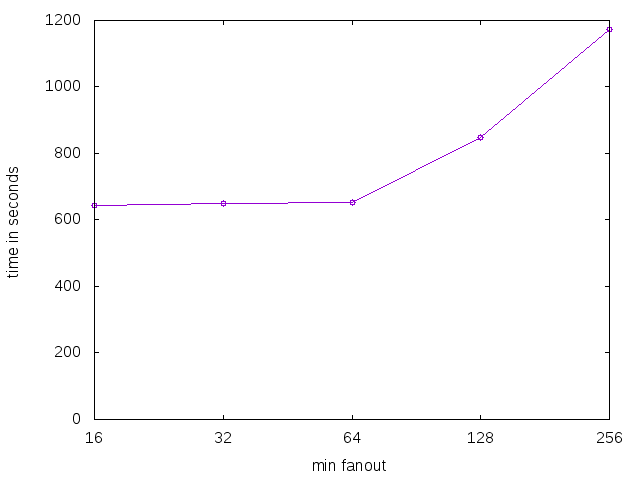
\includegraphics[width=.8\textwidth]{impl/fanout.png}
  \caption{Время работы в зависимости от ветвистости узла}
  \label{pic:fanout}
\end{figure}

Эксперимент повторяется три раза и выбирается время минимальной из попыток. Этот
эксперимент повторялся для разных значений минимальной ветвистости: 16, 32, 64,
128, 256. Результаты эксперимента вы можете увидеть на рисунке~\ref{pic:fanout}.
Как вы можете увидеть, при небольших значениях минимальной ветвистости
результаты отличаются незначительно, но при увеличении ветвистости время
выполнения начинает резко возрастать.

\begin{table}[h]
  \centering
  \begin{subfigure}{.5\textwidth}
    \begin{tabular}{ r l }
        overhead & symbol \\ \hline
        23.29\% & [ctree] XXH64 \\
        21.48\% & [ctree] myfs\_ctree\_it\_find \\
        14.51\% & [kernel] copy\_user\_enhanced\_fast\_string \\
        5.35\%  & [kernel] \_\_radix\_tree\_lookup \\
        3.27\%  & [kernel] find\_get\_entry \\
        2.77\%  & [libc] \_int\_malloc \\
        2.52\%  & [libc] \_int\_free \\
        2.36\%  & [kernel] generic\_file\_read\_iter \\
        2.33\%  & [ctree] ctree\_query\_cmp \\
        1.53\%  & [kernel] entry\_SYSCALL\_64 \\
    \end{tabular}
    \caption{ветвистость 16}
  \end{subfigure}
  \begin{subfigure}{.5\textwidth}
    \begin{tabular}{ r l }
        overhead & symbol \\ \hline
        28.61\% & [ctree] XXH64 \\
        24.20\% & [ctree] myfs\_ctree\_it\_find \\
        17.74\% & [kernel] copy\_user\_enhanced\_fast\_string \\
        4.02\%  & [kernel] \_\_radix\_tree\_lookup \\
        3.18\%  & [kernel] find\_get\_entry \\
        2.61\%  & [kernel] generic\_file\_read\_iter \\
        1.67\%  & [libc] \_int\_malloc \\
        1.42\%  & [libc] \_int\_free \\
        1.40\%  & [ctree] ctree\_query\_cmp \\
        1.11\%  & [libc] \_\_memcmp\_sse4\_1 \\
        0.98\%  & [kernel] copy\_page\_to\_iter \\
        0.93\%  & [kernel] entry\_SYSCALL\_64 \\
    \end{tabular}
    \caption{ветвистость 256}
  \end{subfigure}
  \caption{Результаты профилирования утилитой perf}
  \label{tbl:prof}
\end{table}

Это можно объяснить следующим образом, при небольших значениях минимальной
ветвистости количество элементов в узле определяется размером страницы, однако,
когда элементы перестают помещаться в одну страницу результаты начинают
ухудшаться, так как возрастает время на подсчет хеша прочитанного узла. Это
подтверждается результатами профилирования в таблице~\ref{tbl:prof}. Как вы
можете заметить большая часть времени работы приходится на функцию XXH64,
которая занимается вычислением хеша.

Таким образом при точечных запросах имеет смысл использовать минимально
возможные узлы дерева, чтобы сократить время на подсчет хешей узлов. Однако
ограничивать ветвистость исключительно размером страницы нельзя, так как при
больших размерах элементов с ростом высоты дерева будет ухудшаться
алгоритмическая сложность поиска в таком дереве. Поэтому в качестве минимальной
ветвистости было выбрано число 16 - минимальное из протестированных значений.

Затрат на подсчет хешей прочитанных узлов можно избежать поддерживая кеш узлов.
Так как даже при случайных запросах некоторые узлы будут использоваться довольно
часто\footnote{Например, корень дерева используется всеми запросами, узлы
близкие к корню также могут использоваться довольно часто.}. Однако в текущей
реализации кеширование узлов дерева не реализовано.


\subsection{Синхронизация доступа к LSM-дереву}

Доступ к LSM-дереву контролируется несколькими блокировками:
\begin{itemize}
  \item read/write блокировка mtlock для словарей в памяти;
  \item read/write блокировка sblock для словарей на диске;
  \item блокировка mtx для защиты при выполнении слияния.
\end{itemize}

Read/write блокировка для словарей в памяти используется следующим образом. Все
операции модификации и поиска в словаре в памяти перед чтением указателя на
словарь захватывают блокировку на чтение. После завершения операции блокировка
отпускается. Так как словарь в памяти использует lock-free реализацию
SkipList-а, то никакой посторонней синхронизации эти операции не требуют.

Однако, при слиянии словаря в памяти со словарем на диске нам необходимо
дождаться пока словарь стабилизируется, т. е. все операции вставки будут
завершены, поэтому манипуляции с указателями на словари в памяти выполняются с
mtlock захваченной на запись. Вместо read/write блокировки можно было бы
воспользоваться одним из механизмов безопасного освобождения памяти, но опять же
в целях простоты реализации было принято решение использовать именно блокировку.

Read/write блокировка для словарей на диске используется аналогичным к mtlock
образом. Все операции поиска в дереве, а также операция чтения указателей на
корень дерева захватывают блокировку на чтение. По завершению операции
блокировка отпускается. Однако в отличие от mtlock держать блокировку в течение
всего времени выполнения операции не обязательно, так как в текущей реализации
занятое однажды место никогда не переиспользуется.

Наконец блокировка mtx используется чтобы защитить массив флагов намерения
слияния. Чтобы избежать ситуации когда один и тот же словарь используется в двух
конкурирующих операциях слияния перед выполнением операции необходимо захватить
блокировку mtx, подождать пока флаг намерения соответствующий нужному словарю
обнулиться, после чего выставить этот флаг тем самым показав намерение
использовать данный словарь при выполнении операции слияния. По завершении
операции слияния флаг необходимо обнулить.
